% !TeX root = ../summary-syssec.tex

\section{Side Channel Attacks}
\subsection{Introduction}
Security proofs based on models of system and attacker. Most models do not take
into account the implementation and how it interacts with the environment.

Examples:
\begin{itemize}
  \item Faulty Output (Glitch)
  \item Power Consumption
  \item EM Emissions
  \item Heat
  \item Timing
  \item Design Details
  \item Sound
  \item Data Coupling
\end{itemize}

\textbf{Two categories of Side channel analysis:}
\begin{description}
  \item[Simple] computation only depends upon the key.
  \item[Differential] computation depends upon both the input and the key.
\end{description}

\subsection{Timing Cryptanalysis of RSA}
\begin{enumerate}
  \item Execution time depends on the key
  \item Can be measured for different inputs
\end{enumerate}


\subsubsection{Square-And-Multiply}

\begin{itemize}
  \item Key-dependent Branching
  \item Attacker observes how many 1 are in the key
\end{itemize}
Greatly reduces the search space for the secret key, but still huge...

\subsubsection{Montgomery multiplication}
Multiplication the execution time depends on \textbf{input and key}.

Attack main idea:
\begin{itemize}
  \item Process attack bit per bit.
  \item Try large number of different messages and leverage average execution
    time.
  \item For each message, test whether the round bit was 1 or 0.
\end{itemize}

\subsubsection{Protecting}
\begin{itemize}
  \item Change implementation s.t. it is not time dependent.
  \item Generic protection is hard.
  \item Performance Penalty
\end{itemize}


\subsection{Cache Attacks}
\subsubsection{Prime+Probe}
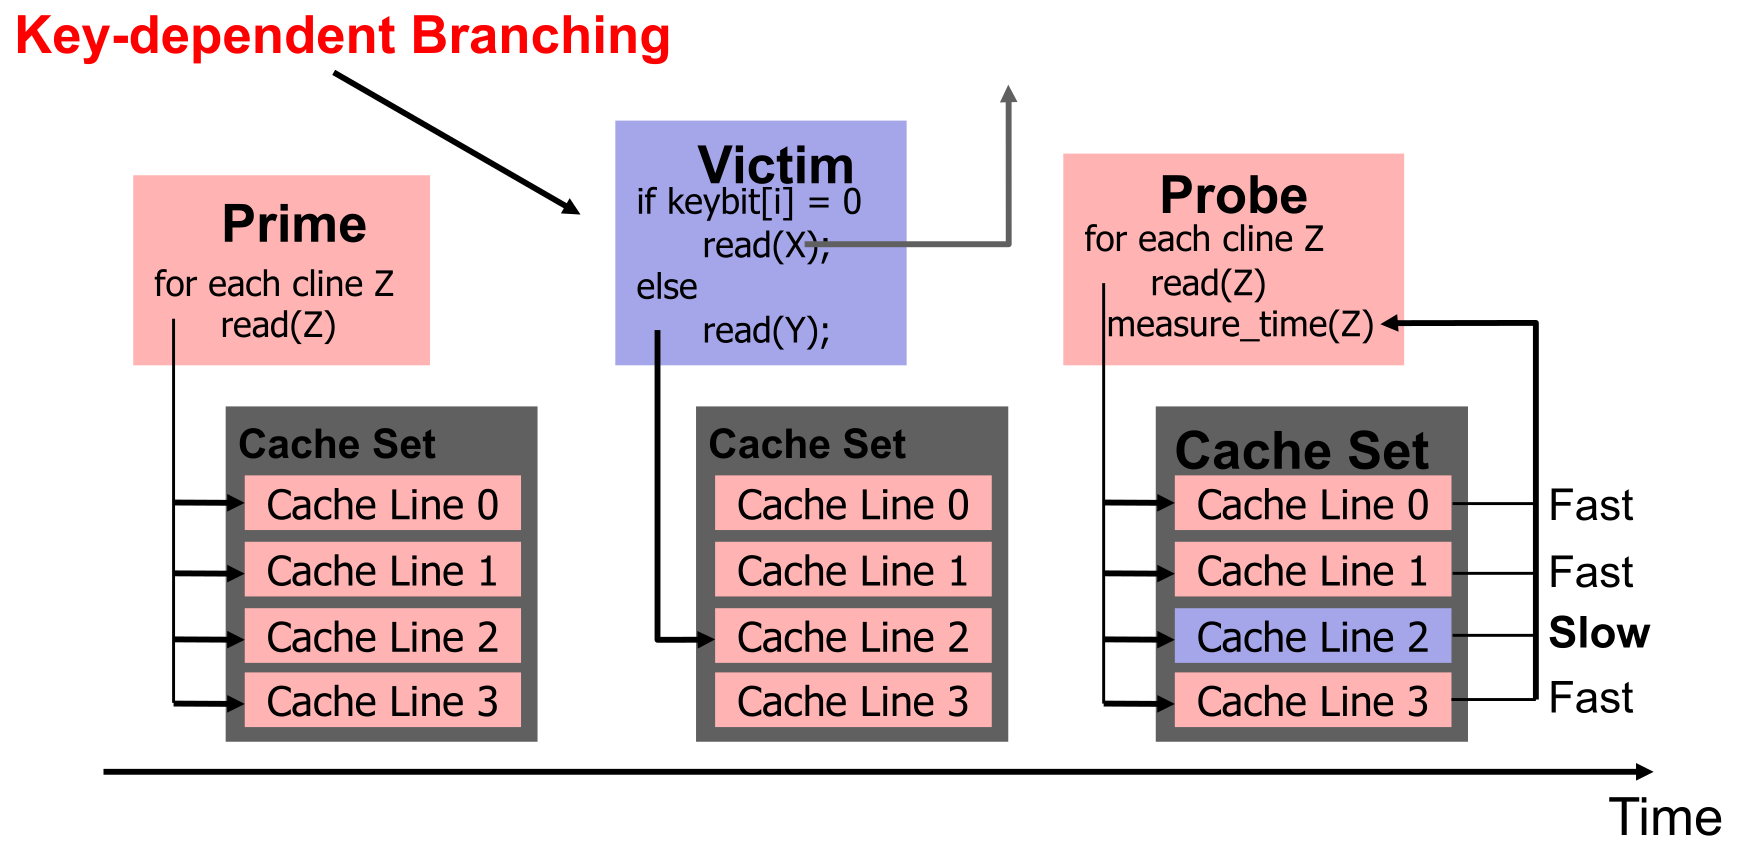
\includegraphics[width=\columnwidth]{sidechannel-prime-probe.png}
\subsubsection{Variants}
\begin{enumerate}
  \item \textbf{Data access} depends on secret data: Data access patterns
    in the cache leak information about the secret
  \item \textbf{Control flow} depends on secret data: Code access
    patterns in the cache leak information about the secret
\end{enumerate}
\subsubsection{Cache Timing Attack on AES}
\textbf{Background}\\
During the execution of AES secret key is used to
index arrays (S-boxes). The time to lookup an array element depends
on whether this element of the S-box has partially or entirely been loaded into the
cache.
\begin{itemize}
  \item Allows complete key recovery.
  \item Problem is in the design, not in the implementation.
\end{itemize}

\textbf{Setting:}
\begin{itemize}
  \item Attacker can send messages and observe overall execution time
  \item Attacker has same setup (software, hardware) for local tests
    Execution
\end{itemize}

\textbf{Attack:}
\begin{itemize}
  \item For each byte of the key, one index value will have the slowest lookup.
  \item The total execution will be slow
  \item Find this index value
  \item (try many messages locally)
\end{itemize}


\subsubsection{Protecting}
\begin{itemize}
  \item \textbf{Basic principle:}
    Try to eliminate secret-dependent cache access patterns
  \item Specific defenses exist, but eliminating all secret-dependent
    branching (code and data) is difficult and expensive…
  \item Most CPUs have special AES hardware  $\Rightarrow$ not vulnerable.
\end{itemize}

\subsection{Power Analysis Attacks}
Mainly used on Smartcards, RFID chips, Sensor Nodes
\begin{itemize}
  \item The attacker needs to have physical access
  \item Measures the consumed power during  operation
\end{itemize}
Square-and-multy in RSA is vulnerable through simple power analysis.
\subsubsection{Protection}
Goal: Elimination or significant reduction of the correlation between operand
values and power consumption.
\begin{itemize}
  \item Random change of power consumption in time
  \item Noise generator
  \item Physical shielding
  \item Software balancing
  \item Hardware balancing
\end{itemize}

\subsection{Acoustic Attacks}
\begin{itemize}
  \item High-frequency sounds caused by vibration of
    electronic components
  \item \textbf{Different keys cause different sounds}
  \item Can extract RSA keys based on sound
\end{itemize}

\subsection{Electromagnetic Attacks}
TEMPEST: Transmitted Electro-Magnetic Pulse / Energy
Standards \& Testing
\begin{itemize}
  \item Compromising emanations may be generated by any electrical information generating or processing equipment.
  \item Can be sensed and transmitted over air, water, electrical lines, ...
  \item Typical examples include:
    \begin{itemize}
      \item Displays
      \item Keyboards
      \item Cables
      \item Processors
    \end{itemize}
\end{itemize}
